\PassOptionsToPackage{unicode=true}{hyperref} % options for packages loaded elsewhere
\PassOptionsToPackage{hyphens}{url}
%
\documentclass[]{article}
\usepackage{lmodern}
\usepackage{amssymb,amsmath}
\usepackage{ifxetex,ifluatex}
\usepackage{fixltx2e} % provides \textsubscript
\ifnum 0\ifxetex 1\fi\ifluatex 1\fi=0 % if pdftex
  \usepackage[T1]{fontenc}
  \usepackage[utf8]{inputenc}
  \usepackage{textcomp} % provides euro and other symbols
\else % if luatex or xelatex
  \usepackage{unicode-math}
  \defaultfontfeatures{Ligatures=TeX,Scale=MatchLowercase}
\fi
% use upquote if available, for straight quotes in verbatim environments
\IfFileExists{upquote.sty}{\usepackage{upquote}}{}
% use microtype if available
\IfFileExists{microtype.sty}{%
\usepackage[]{microtype}
\UseMicrotypeSet[protrusion]{basicmath} % disable protrusion for tt fonts
}{}
\IfFileExists{parskip.sty}{%
\usepackage{parskip}
}{% else
\setlength{\parindent}{0pt}
\setlength{\parskip}{6pt plus 2pt minus 1pt}
}
\usepackage{hyperref}
\hypersetup{
            pdftitle={Yumin Huang's CV},
            pdfauthor={Yumin Huang},
            pdfborder={0 0 0},
            breaklinks=true}
\urlstyle{same}  % don't use monospace font for urls
\usepackage[margin=1in]{geometry}
\usepackage{graphicx,grffile}
\makeatletter
\def\maxwidth{\ifdim\Gin@nat@width>\linewidth\linewidth\else\Gin@nat@width\fi}
\def\maxheight{\ifdim\Gin@nat@height>\textheight\textheight\else\Gin@nat@height\fi}
\makeatother
% Scale images if necessary, so that they will not overflow the page
% margins by default, and it is still possible to overwrite the defaults
% using explicit options in \includegraphics[width, height, ...]{}
\setkeys{Gin}{width=\maxwidth,height=\maxheight,keepaspectratio}
\setlength{\emergencystretch}{3em}  % prevent overfull lines
\providecommand{\tightlist}{%
  \setlength{\itemsep}{0pt}\setlength{\parskip}{0pt}}
\setcounter{secnumdepth}{0}
% Redefines (sub)paragraphs to behave more like sections
\ifx\paragraph\undefined\else
\let\oldparagraph\paragraph
\renewcommand{\paragraph}[1]{\oldparagraph{#1}\mbox{}}
\fi
\ifx\subparagraph\undefined\else
\let\oldsubparagraph\subparagraph
\renewcommand{\subparagraph}[1]{\oldsubparagraph{#1}\mbox{}}
\fi

% set default figure placement to htbp
\makeatletter
\def\fps@figure{htbp}
\makeatother


\title{Yumin Huang's CV}
\author{Yumin Huang}
\date{2021-08-22}

\begin{document}
\maketitle

\hypertarget{aside}{%
\section{Aside}\label{aside}}

\begin{figure}
\centering
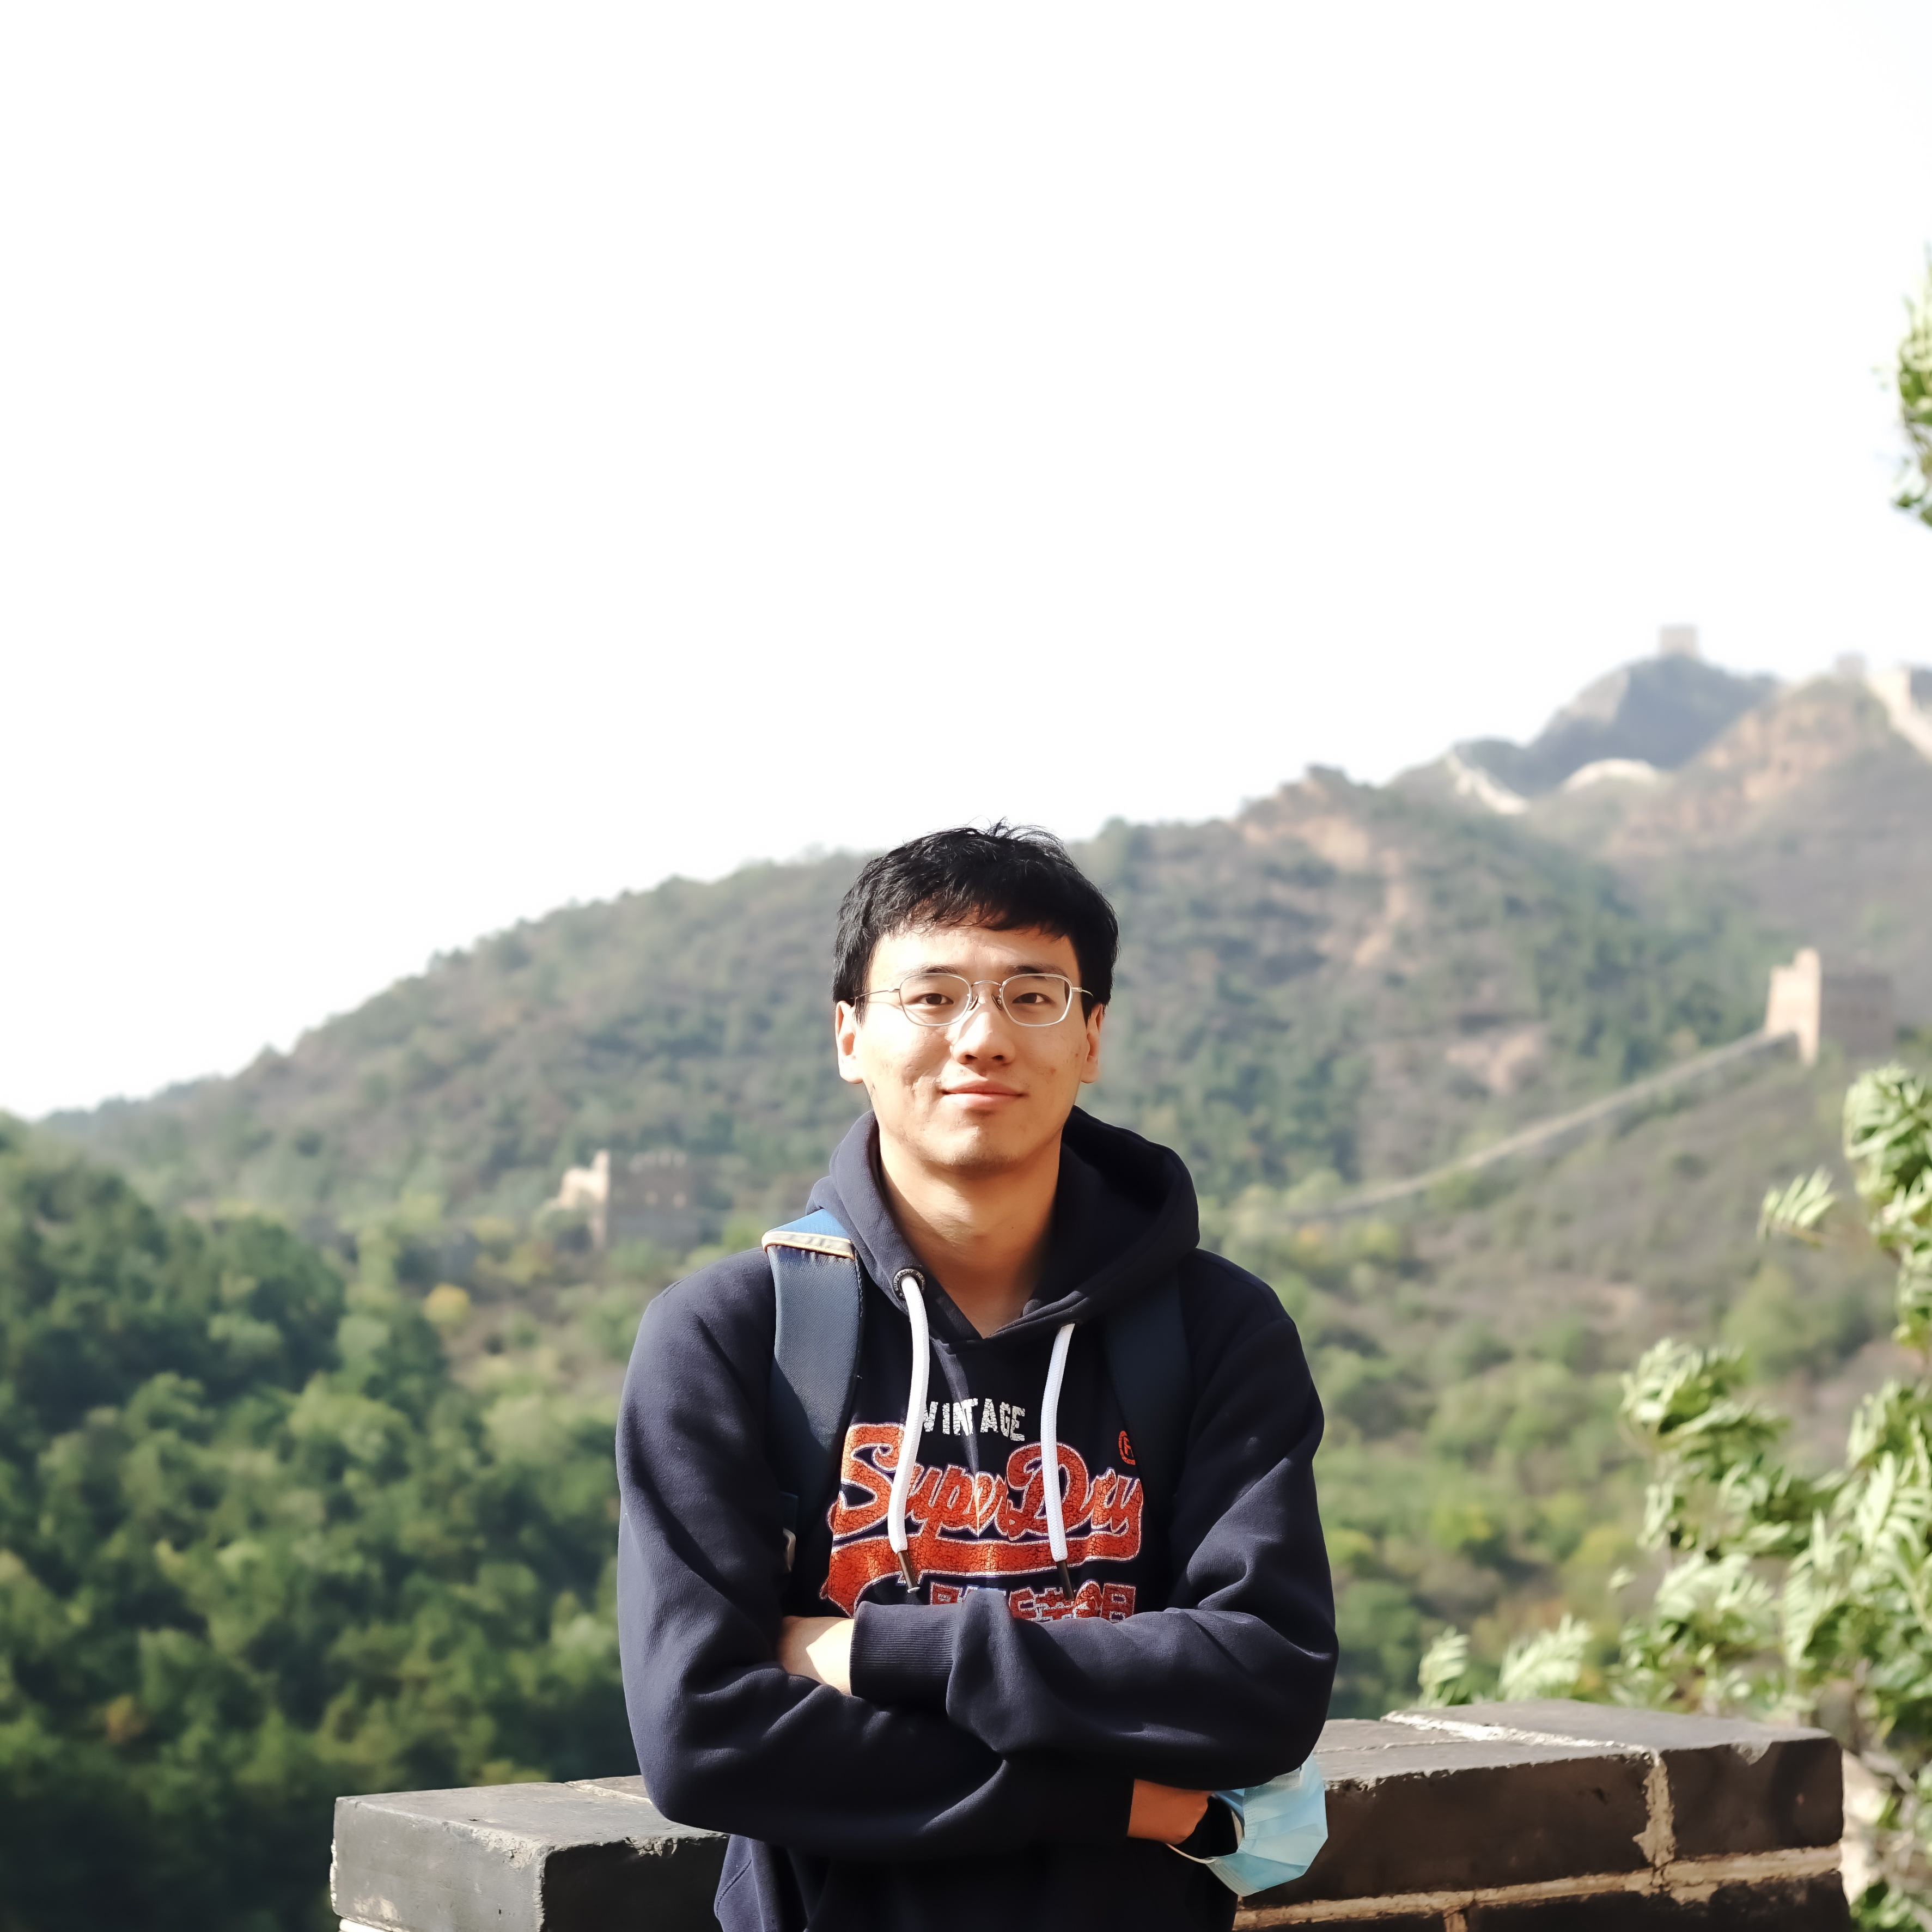
\includegraphics[width=1\textwidth,height=\textheight]{ymhuang.jpeg}
\caption{logo}
\end{figure}

View this CV online with links at \emph{sdws1983.github.io/cv}

\hypertarget{contact}{%
\subsection{Contact 联系方式}\label{contact}}

\begin{itemize}
\tightlist
\item
   \href{mailto:ymhuang@cau.edu.cn}{\nolinkurl{ymhuang@cau.edu.cn}}
\item
   github.com/sdws1983
\item
   \url{https://sdws1983.github.io/}
\item
   (86) 15652920371
\end{itemize}

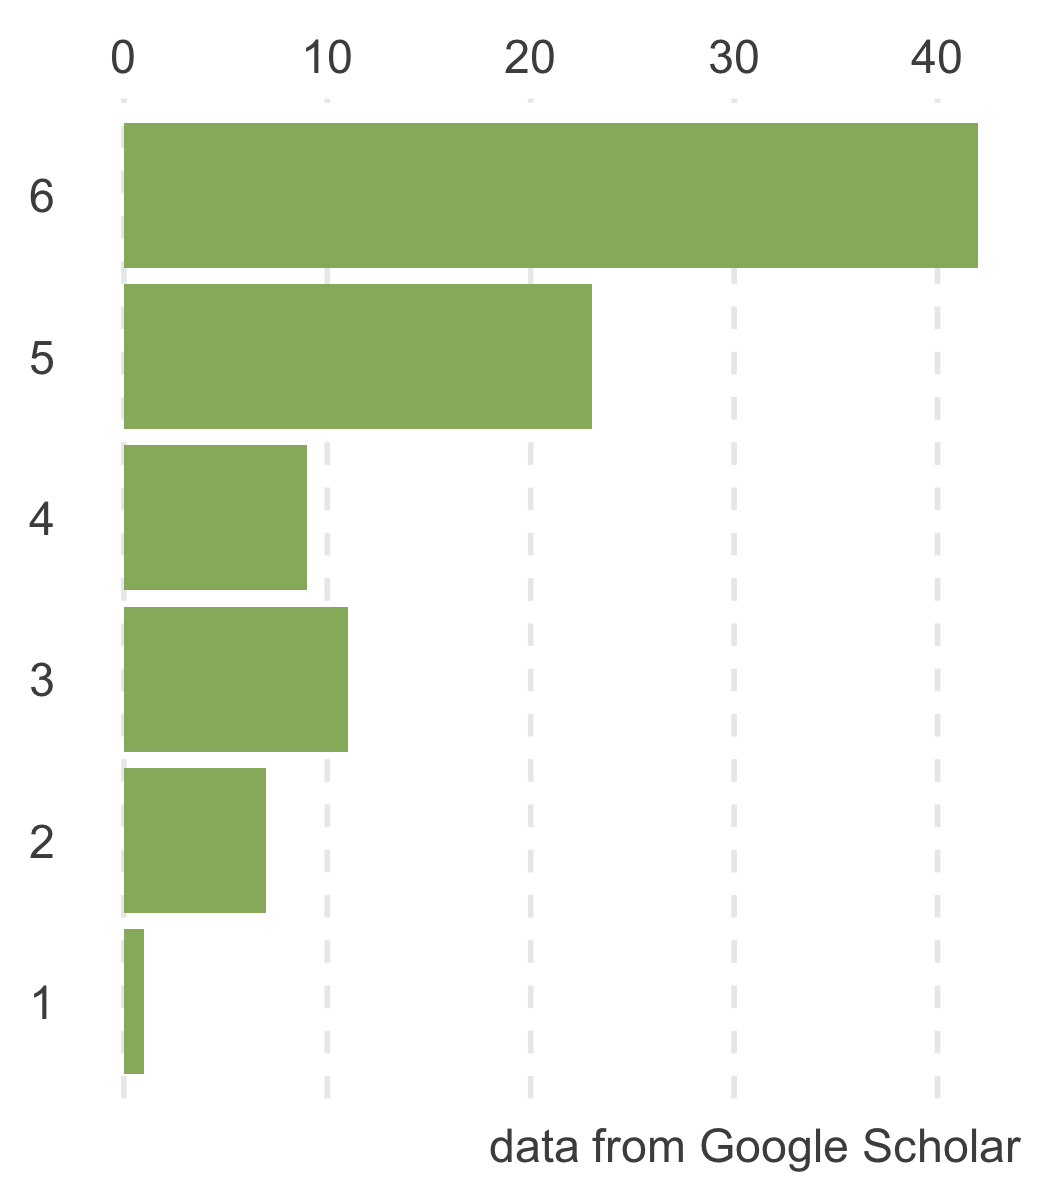
\includegraphics{citation.png}

\hypertarget{disclaimer}{%
\subsection{Disclaimer}\label{disclaimer}}

Last updated on 2021-08-22.

\hypertarget{main}{%
\section{Main}\label{main}}

\hypertarget{title}{%
\subsection{黄育敏 Yumin Huang}\label{title}}

PhD candidate of Crop genetics and breeding at
\href{http://www.cau.edu.cn/}{China Agricultural University}.

中国农业大学,作物遗传育种专业博士.

I am broadly interested in plant genomics, comparative genomics,
molecular evolution, epigenomics, 3D genomics, bioinformatics, data
integration and visualization.

本人对植物基因组学,比较基因组学,分子进化,表观遗传学,三维基因组学,生物信息学,数据处理及可视化等方面有着广泛兴趣。

\hypertarget{education-ux6559ux80b2ux7ecfux5386}{%
\subsection{Education
教育经历}\label{education-ux6559ux80b2ux7ecfux5386}}

\hypertarget{phd.-crop-genetics-and-breeding-ux4f5cux7269ux9057ux4f20ux80b2ux79cdux4e13ux4e1a-ux535aux58eb}{%
\subsubsection{PhD., Crop genetics and breeding 作物遗传育种专业,
博士}\label{phd.-crop-genetics-and-breeding-ux4f5cux7269ux9057ux4f20ux80b2ux79cdux4e13ux4e1a-ux535aux58eb}}

China Agricultural University 中国农业大学

Beijing, CN

2022 - 2016

\hypertarget{b.s.-biotechnology-ux751fux7269ux6280ux672fux4e13ux4e1a-ux5b66ux58eb}{%
\subsubsection{B.S., Biotechnology 生物技术专业,
学士}\label{b.s.-biotechnology-ux751fux7269ux6280ux672fux4e13ux4e1a-ux5b66ux58eb}}

Beijing Forestry University 北京林业大学

Beijing, CN

2016 - 2012

\hypertarget{scholarships-awards-ux5956ux52b1ux8363ux8a89}{%
\subsection{Scholarships \& Awards
奖励荣誉}\label{scholarships-awards-ux5956ux52b1ux8363ux8a89}}

\hypertarget{ux535aux58ebux7814ux7a76ux751fux56fdux5bb6ux5956ux5b66ux91d1}{%
\subsubsection{博士研究生国家奖学金}\label{ux535aux58ebux7814ux7a76ux751fux56fdux5bb6ux5956ux5b66ux91d1}}

中华人民共和国教育部

N/A

2020

\hypertarget{ux5b66ux672fux6c47ux62a5ux4e8cux7b49ux5956}{%
\subsubsection{学术汇报二等奖}\label{ux5b66ux672fux6c47ux62a5ux4e8cux7b49ux5956}}

国家玉米改良中心年度论坛

N/A

\hypertarget{ux535aux58ebux4e00ux7b49ux5956ux5b66ux91d1}{%
\subsubsection{博士一等奖学金}\label{ux535aux58ebux4e00ux7b49ux5956ux5b66ux91d1}}

中国农业大学

N/A

2019

\hypertarget{ux535aux58ebux4e8cux7b49ux5956ux5b66ux91d1}{%
\subsubsection{博士二等奖学金}\label{ux535aux58ebux4e8cux7b49ux5956ux5b66ux91d1}}

中国农业大学

N/A

2018

\hypertarget{publications-ux53d1ux8868ux6587ux7ae0}{%
\subsection{Publications
发表文章}\label{publications-ux53d1ux8868ux6587ux7ae0}}

\hypertarget{megabase-scale-presence-absence-variation-with-tripsacum-origin-was-under-selection-during-maize-domestication-and-adaptation}{%
\subsubsection{\texorpdfstring{\href{https://doi.org/10.1186/s13059-021-02448-2}{Megabase-scale
presence-absence variation with \emph{Tripsacum} origin was under
selection during maize domestication and
adaptation}}{Megabase-scale presence-absence variation with Tripsacum origin was under selection during maize domestication and adaptation}}\label{megabase-scale-presence-absence-variation-with-tripsacum-origin-was-under-selection-during-maize-domestication-and-adaptation}}

\textbf{\emph{Genome Biology}}. 2021, 22(1):237.

N/A

2021

\begin{itemize}
\tightlist
\item
  \textbf{Huang, Y.}\textsuperscript{\#}, Huang, W.\textsuperscript{\#},
  Meng, Z., Braz, G. T., Li, Y., Wang, K., Wang, H., Lai, J., Jiang, J.,
  Dong, Z.\textsuperscript{*}, \& Jin, W.\textsuperscript{*} (第一作者)
\end{itemize}

\hypertarget{evolution-and-domestication-footprints-uncovered-from-the-genomes-of-coix}{%
\subsubsection{\texorpdfstring{\href{http://dx.doi.org/10.1016/j.molp.2019.11.009}{Evolution
and Domestication Footprints Uncovered from the Genomes of
\emph{Coix}}}{Evolution and Domestication Footprints Uncovered from the Genomes of Coix}}\label{evolution-and-domestication-footprints-uncovered-from-the-genomes-of-coix}}

\textbf{\emph{Molecular Plant }}. 2019, 13(2):295-308.

N/A

2019

\begin{itemize}
\tightlist
\item
  Liu, H.\textsuperscript{\#}, Shi, J.\textsuperscript{\#}, Cai,
  Z.\textsuperscript{\#}, \textbf{Huang, Y.}\textsuperscript{\#}, Lv,
  M., Du, H., Gao, Q., Zuo, Y., Dong, Z., Huang, W., Qin, R., Liang, C.,
  Lai, J.\textsuperscript{*} , \& Jin, W\textsuperscript{*} .
  (共同第一作者)
\end{itemize}

\hypertarget{male-sterile-28-encodes-an-argonaute-family-protein-essential-for-male-fertility-in-maize}{%
\subsubsection{\texorpdfstring{\href{_https://doi.org/10.1007/s10577-021-09653-6}{\emph{Male
sterile} 28 encodes an ARGONAUTE family protein essential for male
fertility in
maize}}{Male sterile 28 encodes an ARGONAUTE family protein essential for male fertility in maize}}\label{male-sterile-28-encodes-an-argonaute-family-protein-essential-for-male-fertility-in-maize}}

\textbf{\emph{Chromosome Research}}. 2021, 29(2):189\_201

N/A

2021

\begin{itemize}
\tightlist
\item
  Li, Y., \textbf{Huang, Y.}, Pan, L., Zhao, Y., Huang,
  W.\textsuperscript{*}, \& Jin, W.\textsuperscript{*}
\end{itemize}

\hypertarget{a-missense-mutation-in-a-large-subunit-of-ribonucleotide-reductase-confers-temperature-gated-tassel-formation}{%
\subsubsection{\texorpdfstring{\href{https://doi.org/10.3389/fimmu.2021.687975}{A
missense mutation in a large subunit of ribonucleotide reductase confers
temperature-gated tassel
formation}}{A missense mutation in a large subunit of ribonucleotide reductase confers temperature-gated tassel formation}}\label{a-missense-mutation-in-a-large-subunit-of-ribonucleotide-reductase-confers-temperature-gated-tassel-formation}}

\textbf{\emph{Plant Physiology}}. 2020, 184(4):1979\_1997

N/A

2020

\begin{itemize}
\tightlist
\item
  Xie, S.\textsuperscript{\#}, Luo, H.\textsuperscript{\#},
  \textbf{Huang, Y.}, Wang, Y., Ru, W., Shi, Y., Huang, W., Wang, H.,
  Dong, Z., \& Jin, W.\textsuperscript{*}
\end{itemize}

\hypertarget{dlf1-promotes-floral-transition-by-directly-activating-zmmads4-and-zmmads67-in-the-maize-shoot-apex}{%
\subsubsection{\texorpdfstring{\href{https://dx.doi.org/10.1111/nph.16772}{\emph{dlf1}
promotes floral transition by directly activating \emph{ZmMADS4} and
\emph{ZmMADS67} in the maize shoot
apex}}{dlf1 promotes floral transition by directly activating ZmMADS4 and ZmMADS67 in the maize shoot apex}}\label{dlf1-promotes-floral-transition-by-directly-activating-zmmads4-and-zmmads67-in-the-maize-shoot-apex}}

\textbf{\emph{New Phytologist}}. 2020, 228(4):1386-1400.

N/A

\begin{itemize}
\tightlist
\item
  Sun, H.\textsuperscript{\#}, Wang, C.\textsuperscript{\#}, Chen, X.,
  Liu, H., \textbf{Huang, Y.}, Li, S., Dong, Z., Zhao, X., Tian,
  F.\emph{\textsuperscript{*}, \& Jin, W.}\textsuperscript{*}
\end{itemize}

\hypertarget{maize-male-sterile-33-encodes-a-putative-glycerol-3-phosphate-acyltransferase-that-mediates-anther-cuticle-formation-and-microspore-development}{%
\subsubsection{\texorpdfstring{\href{https://doi.org/10.1186/s12870-018-1543-7}{Maize
\emph{male sterile 33} encodes a putative glycerol-3-phosphate
acyltransferase that mediates anther cuticle formation and microspore
development}}{Maize male sterile 33 encodes a putative glycerol-3-phosphate acyltransferase that mediates anther cuticle formation and microspore development}}\label{maize-male-sterile-33-encodes-a-putative-glycerol-3-phosphate-acyltransferase-that-mediates-anther-cuticle-formation-and-microspore-development}}

\textbf{\emph{BMC Plant Biology}}. 2018, 18(1).

N/A

2018

\begin{itemize}
\tightlist
\item
  Zhang, L.\textsuperscript{\#}, Luo, H.\textsuperscript{\#}, Zhao,
  Y.\textsuperscript{\#}, Chen, X., \textbf{Huang, Y.}, Yan, S., Li, S.,
  Liu, M., Huang, W., Zhang, X., \& Jin, W.*\textsuperscript{*}
\end{itemize}

\hypertarget{leaf-extract-from-lithocarpus-polystachyus-rehd.-promote-glycogen-synthesis-in-t2dm-mice}{%
\subsubsection{\texorpdfstring{\href{https://dx.doi.org/10.1371/journal.pone.0166557}{Leaf
extract from \emph{Lithocarpus polystachyus} Rehd. Promote glycogen
synthesis in T2DM
mice}}{Leaf extract from Lithocarpus polystachyus Rehd. Promote glycogen synthesis in T2DM mice}}\label{leaf-extract-from-lithocarpus-polystachyus-rehd.-promote-glycogen-synthesis-in-t2dm-mice}}

\textbf{\emph{PLoS ONE}}. 2016, 11(11).

N/A

2016

\begin{itemize}
\tightlist
\item
  Wang, J.\textsuperscript{\#}, \textbf{Huang, Y.}\textsuperscript{\#},
  Li, K.\textsuperscript{\#}, Chen, Y., Vanegas, D., McLamore, E. S., \&
  Shen, Y.*\textsuperscript{*} (共同第一作者)
\end{itemize}

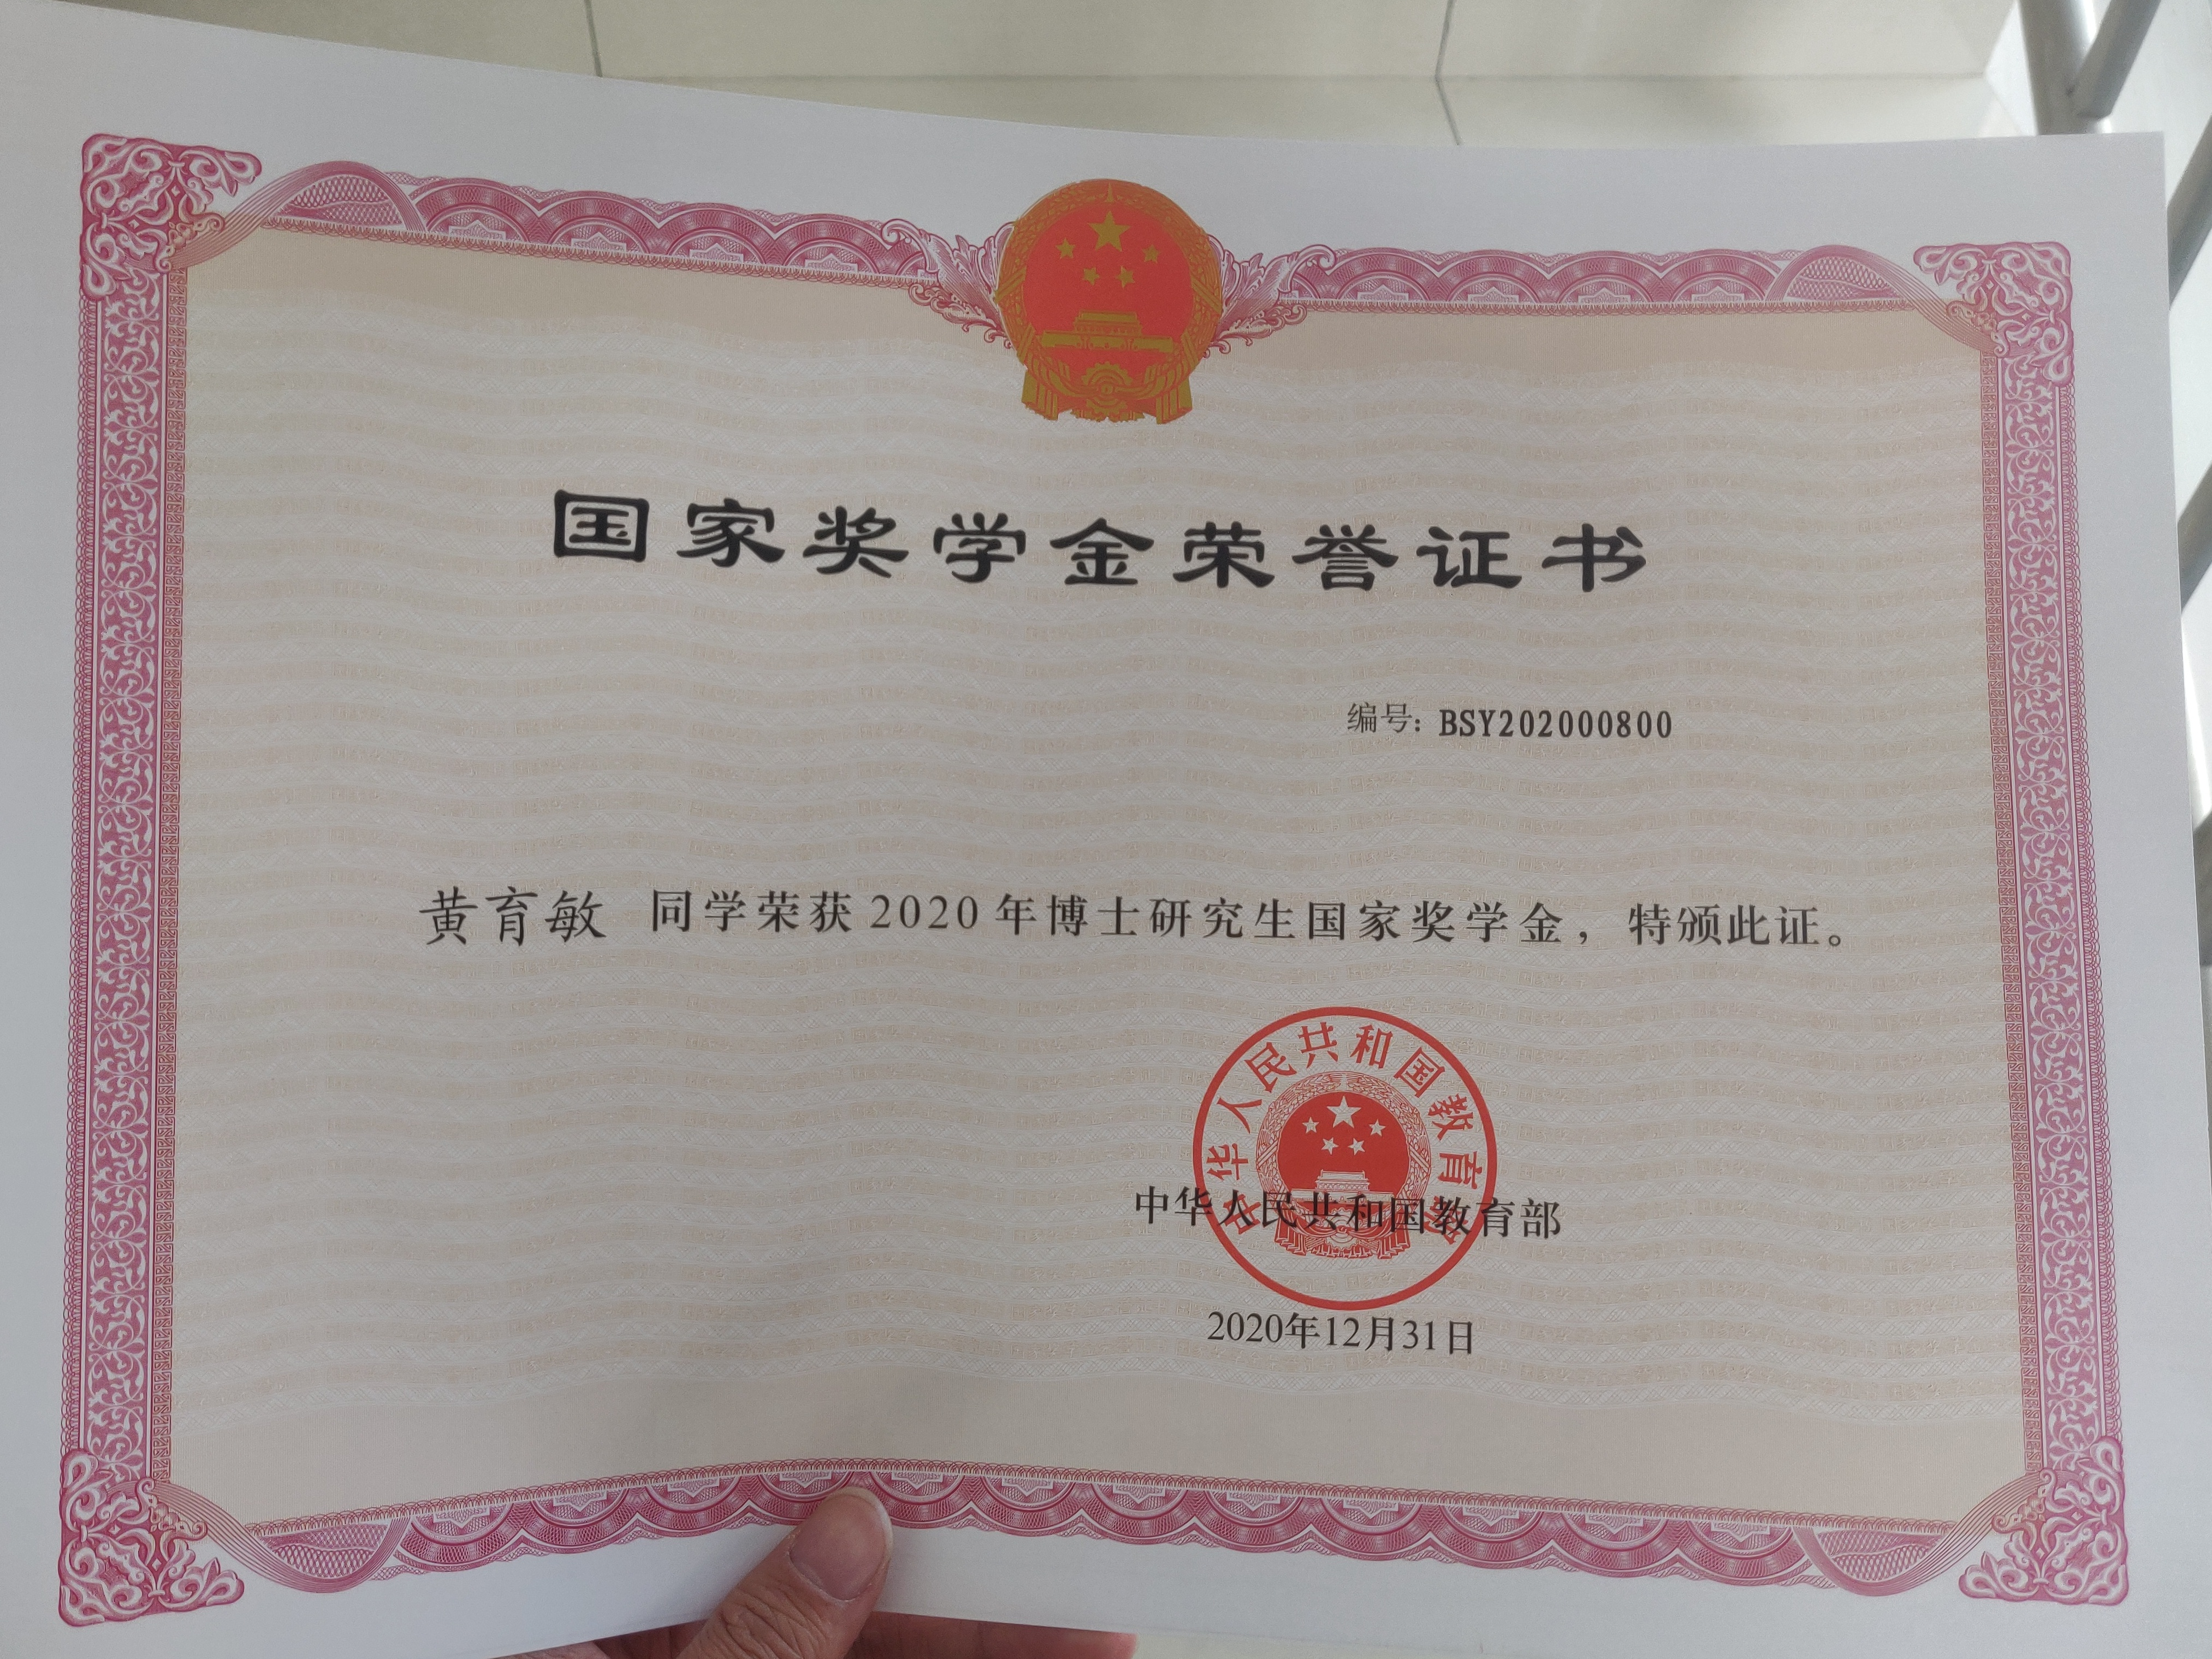
\includegraphics[width=1\textwidth,height=\textheight]{figures/guojiang.jpeg}

\end{document}
